\section{Django}

Django es un framework de desarrollo web de código abierto, escrito en Python,
que respeta el paradigma conocido como {\bfseries Model Template View}. Fue desarrollado en
origen para gestionar varias páginas orientadas a noticias de la
{\bfseries World Company de Lawrence, Kansas}, y fue liberada al público bajo una licencia
BSD en julio de 2005; el framework fue nombrado en alusión al guitarrista de
jazz gitano Django Reinhardt \url{http://es.wikipedia.org/wiki/Django_Reinhardt}.

En junio del 2008 fue anunciado que la recién formada Django Software Foundation
se haría cargo de Django en el futuro.

La meta fundamental de Django es facilitar la creación de sitios web complejos.
Django pone énfasis en el re-uso, la conectividad y extensibilidad de
componentes, el desarrollo rápido y el principio No te repitas
(DRY, del inglés Don't Repeat Yourself). Python es usado en todas las partes
del framework, incluso en configuraciones, archivos, y en los modelos de datos.


\subsection{MVC}

Antes de Explicar como funciona Django empezare por una breve explicacion de
el patr\'on (MVC) Modelo Vista Controlador el cual es un patrón de arquitectura de software que
separa los datos y la lógica de negocio de una aplicación de la interfaz de
usuario y el módulo encargado de gestionar los eventos y las comunicaciones.
Para ello MVC propone la construcción de tres componentes distintos que son el
modelo, la vista y el controlador, es decir, por un lado define componentes
para la representación de la información, y por otro lado para la interacción
 del usuario. Este patrón de diseño se basa en las ideas de reutilización de
 código y la separación de conceptos, características que buscan facilitar la
 tarea de desarrollo de aplicaciones y su posterior mantenimiento.

De manera genérica, los componentes de MVC se podrían definir como sigue:

{\bfseries  El Modelo:} Es la representación de la información con la cual el sistema opera,
por lo tanto gestiona todos los accesos a dicha información, tanto consultas
como actualizaciones, implementando también los privilegios de acceso que se
hayan descrito en las especificaciones de la aplicación (lógica de negocio).
Envía a la 'vista' aquella parte de la información que en cada momento se le
solicita para que sea mostrada (típicamente a un usuario). Las peticiones de
acceso o manipulación de información llegan al 'modelo' a través del
'controlador'.

{\bfseries El Controlador: } Responde a eventos (usualmente acciones del
usuario) e invoca peticiones al 'modelo' cuando se hace alguna solicitud sobre
la información (por ejemplo, editar un documento o un registro en una base de
datos). También puede enviar comandos a su 'vista' asociada si se solicita un
cambio en la forma en que se presenta de 'modelo' (por ejemplo, desplazamiento
 o scroll por un documento o por los diferentes registros de una base de datos),
  por tanto se podría decir que el 'controlador' hace de intermediario entre
   la 'vista' y el 'modelo' actuando como Middleware
\footnote{Middleware es el software que proporciona un enlace entre aplicaciones de software
independientes. Middleware a veces se llama a la vía que conecta dos
aplicaciones y pasa los datos entre ellas. Los Middleware permiten que los
datos contenidos en una base de datos puedan ser accedidos a través de otra.
Ahorra el tiempo a los programadores.}.
   
{\bfseries La Vista: } Presenta el 'modelo' (información y lógica de negocio)
 en un formato adecuado para interactuar (usualmente la interfaz de usuario)
 por tanto requiere de dicho 'modelo' la información que debe representar como
 salida.

\begin{figure}[h]
    \centering
    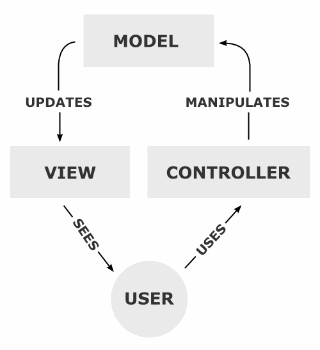
\includegraphics[scale=0.7]{resourse/MVC-Process.png}
    \caption{Diagrama del Patron MVC Modelo Vista Controlador}
    \label{fig:03}
\end{figure}    


\subsection{Django y el MVT}

Si hicieramos una clasificacion de Herramientas de desarrollo web, podriamos
clasificar a Django como parte de la tercera generacion:


\begin{figure}[h]
    \centering
    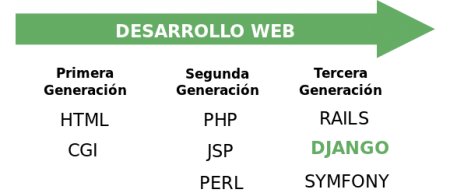
\includegraphics[scale=0.7]{resourse/desarrolloweb.png}
    \caption{Generaciones de Herramientas de Desarrollo Web}
    \label{fig:02}
\end{figure}   

Sin embargo más alla de las clasificaciones que podr\'ian existir, está el
entender como funciona realmente, al entenderlo se puede llegar a dominarlo.

Dijimos que era un framework MTV (una modificación de MVC, nada que ver con
un canal de m\'usica), esto se debe a que los desarrolladores no tuvieron la
 intención de seguir algún patron de desarrollo, sino hacer el framework lo
más funcional posible.

\begin{itemize}
    \item {\bfseries  El Modelo} en Django sigue siendo el modelo
    \item {\bfseries La Vista} en Django se llama Plantilla (Template)
    \item {\bfseries El controlador} en Django se llama Vista
\end{itemize}

Una imagen nos hará entender mejor esta relación:

\begin{figure}[h]
    \centering
    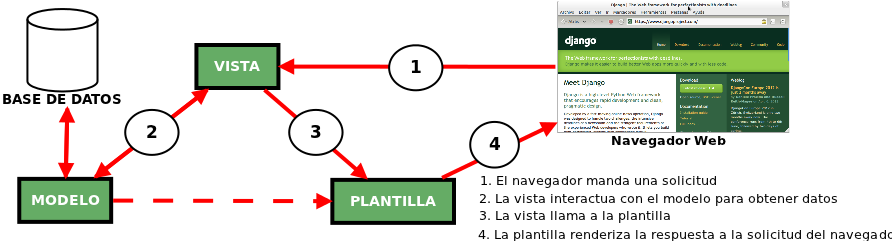
\includegraphics[scale=0.5]{resourse/esquema-mtv.png}
    \caption{El patron Modelo Vista Template de Django}
    \label{fig:04}
\end{figure}   



\subsection{El Modelo}
El modelo define los datos almacenados, se encuentra en forma de clases de
Python, las clases definidas son traducidas por Django y este genera las Tablas
necesarias para el funcionamiento del modelo dentro de la base de datos, cada
tipo de dato que debe ser almacenado se encuentra en una variable 
con ciertos parámetros, posee métodos también. Todo esto permite indicar y
controlar el comportamiento de los datos.\\[0.1cm]

Aqui un extracto del codigo mostrando como se implementa uno de los tantos
modelos con los que trabaja el Sistema\\[0.3cm]


\begin{lstlisting}[style=Python]

class Message(models.Model):
    """
        Clase Para Manejar mensajes entre usuarios
    """
    from_user = models.ForeignKey(User, related_name='from_user')
    to_user = models.ForeignKey(User, related_name='to_user')
    date = models.DateTimeField("Fecha y Hora",auto_now_add=True)
    issue = models.CharField("Asunto",max_length=125, default='')
    content = models.TextField("Cuerpo del Mensaje")
    read = models.BooleanField("Leido",default=False)


    class Meta:
        db_table = "Messages"
        verbose_name = "InboxMessage"
        verbose_name_plural = "InboxMessages"
\end{lstlisting}

\footnote{Como algunos lo notaran la variable from\_user del modelo internamente
es una relacion 1:M dentro de la base de datos.}

\footnote{La Clase interna Meta define atributos expeciales como 'db\_name' que hace
referencia a como se llamara la tabla dentro de la Bases de Datos.}

\vspace{0.1cm}

\subsection{La Vista}
La vista se presenta en forma de funciones en Python, su propósito es
determinar que datos serán visualizados, entre otras cosas más que iremos
viendo conforme avanzamos con el curso. El ORM de Django permite escribir
código Python en lugar de SQL para hacer las consultas que necesita la vista.
La vista también se encarga de tareas conocidas como el envío de correo
electrónico, la autenticación con servicios externos y la validación de
datos a través de formularios. Lo mas importante a entender con respecto a la
 vista es que no tiene nada que ver con el estilo de presentación de los
 datos, sólo se encarga de los datos, la presentación es tarea de la plantilla.\\[0.1cm]


Aqui muestro una vista sencilla que realiza una consulta base de datos que listara todos
los usuarios que sean medicos. \\[0.1cm]

\begin{lstlisting}[style=Python]
def patient_show_medics_list(request):
    """
        Muestra el listado de Medicos
    """
    mi_template = get_template('Patients/GestionTurnos/medics-list.html')
    dict = generate_base_keys(request)

    if is_patient(request.user):
        dict['medics'] = UserInformation.objects.filter( \\
                                    user__groups__name='Medico')
        html_cont = mi_template.render(Context(dict))
        return HttpResponse(html_cont)

    else:
        #si hay un usuario logueado intentanto acceder sera enviado a una
        # pagina de error
        path = request.META['PATH_INFO']
        return HttpResponseRedirect("/restricted-access%s" %path)
\end{lstlisting}

\vspace{0.1cm}

Aunque es un ejemplo sencillo podemos apreciar el potencial de Django, como vemos
no vemos ningun codigo SQL, pues bien dicho codigo SQL se ejecuta internamente
nos aleja del problema de las restriciones de la Base de Datos ya sea que usemos
PosgreSQL (como en este sistema), MySQL, SQLServer o SQLite nosotros
solo escribiremos codigo Python, El framework se encargargara de traducir esa
instrucion al motor de bases de datos correspondiente que estemos usando.\\[0.2cm]

\begin{lstlisting}[style=consola]
dict['medics'] = UserInformation.objects.filter( \\
                            user__groups__name='Medico')
\end{lstlisting}

\vspace{0.1cm}

Traducido a SQL terminariamos con algo tan orrible como esto:\\[0.1cm]

\begin{lstlisting}[style=consola]
SELECT * FROM UserInformation as Info
INNER JOIN User ON Info.username = User.username
INNER JOIN GroupsByUsers ON User.username = GroupsByUsers.username
...
\end{lstlisting}

\vspace{0.1cm}

\subsection{La Plantilla}
La plantilla es básicamente una página HTML con algunas etiquetas extras
propias de Django, en si no solamente crea contenido en HTML (también XML, CSS,
Javascript, CSV, etc).\\[0.1cm]

La plantilla recibe los datos de la vista y luego los organiza para la
presentación al navegador web. Las etiquetas que Django usa para las plantillas
permiten que sea flexible para los
diseñadores del frontend, pueden Extenderse a partir de otras plantillas incluso
tiene estructuras de datos como if, por por si es necesaria una presentación
lógica de los datos, estas estructuras
son límitadas para evitar un desorden poniendo cualquier tipo de código Python.\\[0.1cm]

Esto permite que la lógica del sistema siga permaneciendo en la vista. Aqui la
vista para Iniciar Session:\\[0.1cm]

\begin{lstlisting}[style=HTML]



<link type="text/css" rel="stylesheet" media="all"
    href="/media/css/fancy-forms.css" />
<link type="text/css" rel="stylesheet" media="all"
    href="/media/css/gradient-buttons.css" />
<link type="text/css" rel="stylesheet" media="all"
    href="/media/css/messages.css" />




<br /><br /><br />
        
            <div class="fancy-form-white" style="width: 350px;
                margin: 0 auto;">
                <h3 class="title">Inciar Session</h3><br />
                <form action="." method="POST">
                <table style="margin: 0 auto; width: 330px;" >
                <tr>
                    <td><label for="username">Usuario:</label></td>
                    <td><input type="text" name="username" value=""
                    tabindex="1" id="username"></td>
                    <td rowspan="2">
                    <input type="submit" value="Login" tabindex="3"
                    class="grad-button-blue" style="height: 50px;">
                    </td>
                </tr>
                <tr>
                    <td><label for="password">Contrase\~na:</label></td>
                    <td><input type="password" name="password" value=""
                     tabindex="2" id="password"></td>
                </tr>
                </table>
                </form>
                <br />
            </div>

            
                    <br />
                    <br />
                <div class="alert">Alerta: Error Usuario y/o Contrase\~na
                Incorrectos</div>
            

        
            <div class="alert">Alerta: Usted ya ha iniciado session con el
            usuario <strong>{{ username }}</strong></div>
            <br />
            <a href="/logout">Cerrar Session</a>
        

\end{lstlisting}

\vspace{0.1cm}

\subsection{La Configuracion de Rutas}

Django posee un mapeo de URLs que permite controlar el despliegue de las vistas,
esta configuración es conocida como URLConf. El trabajo del URLConf es leer
la URL que el usuario solicitó, encontrar la vista apropiada para la solicitud
y pasar cualquier variable que la vista necesite para completar su trabajo. El
URLConf esta construido con expresiones regulares en Python y sigue la filosofia
de Python: Explicito es mejor que implícito. Este URLConf permite que las rutas
que maneje Django seán agradables y entendibles para el usuario.\\[0.1cm]

Fragmento del archivo urls.py del Proyecto\\[0.1cm]

\begin{lstlisting}[style=HTML]
    (r'^$', base_views.index),
    (r'^index/$', base_views.index),
    (r'^login/$', base_views.login),
    (r'^logout/$', base_views.logout),
    (r'^change-password/$', base_views.change_password),
    (r'^restricted-access/$', base_views.restricted_access),
    (r'^restricted-access/(.+)/$', base_views.restricted_access),
\end{lstlisting}

\vspace{0.1cm}


\subsection{Instalar Django}

Puedes bajarte Django desde el siguiente enlace \url{https://www.djangoproject.com/download/1.3.7/tarball/}
\footnote {la version 1.3.7 no es la ultima version disponible a la hora de crear
este informe estaba por la 1.6.2 ya que Django se actualiza constantemente.}
te descargara un paquete llamado Django-1.3.7.tar.gz lo descomprimes en
algun directorio luego abres la Terminal y te posicionas sobre el directorio
donde descomprimiste y ejecutas:

\begin{lstlisting}[style=consola]
    $ python setup.py install 
\end{lstlisting}
\vspace{0.1cm}

Sino mediante el instalador de Paquetes de Python de manera mas automatica escribes
en la terminal

\begin{lstlisting}[style=consola]
     pip install django==1.3.7
\end{lstlisting}
\vspace{0.1cm}

Con esto ya tendremos instalado Django.

\section{Instalando el Resto de Las Dependencias}

Ademas de Django en el Proyecto se utilizaron otras Librerias de Python las cuales
algunas vienen instaladas y Otras Requieren ser instaladas de manera similar
a como instalamos Django.

\subsection{psycopg2}

psycopg2 es un adaptador de base de datos PostgreSQL para el lenguaje de
programación Python. psycopg2 fue escrito con el objetivo de ser muy pequeño
y rápido y estable. 

psycopg2 es diferente del otro adaptador de base de datos, ya que fue diseñado
para aplicaciones en gran medida de subprocesos múltiples que crean y destruyen
un montón de cursores y hacen que un número notable de inserciones o
actualizaciones concurrentes. psycopg2 también proporcionan operaciones
asincrónicas completos y apoyo a las bibliotecas de co-rutinas. 

Para instalar descargue el precompilado desde \url{http://www.stickpeople.com/projects/python/win-psycopg/}
Ejecutelo con permisos de administrador, nos pedira que selecionemos la version
de python con que se instalar.

\subsection{ReportLab}

ReportLab es la ultra-robusto motor de código abierto a prueba de tiempo para
la creación de documentos PDF y gráficos vectoriales personalizado. Escrito en
Python, ReportLab es rápido, flexible y una plataforma cruzada.
 
Proporciona un completo conjunto de herramientas de programación para la
creación de documentos y gráficos complejos. Ofrecemos una serie de componentes
 de forma gratuita y de código abierto, además de un paquete comercial con
características adicionales.

Para Instalar descargue el instalado desde \url{http://www.reportlab.com/software/installation/}
y proceda de manera similar a como hizo con la instalacion de psycopg2.


\subsection{easy\_thumbnails}

Easy\_Thumbnails es Una potente aplicación thumbnailing \footnote{Cuando hablamos de thumbnails 
nos referimos a las diferentes miniaturas que son versiones en distintos tamaños
 de una imágen y son usadas para ayudar a su organización y reconocimiento.},
pero fácil de implementacion para Django.

Para Instalar solo ejecute el siguiente comando en terminal, no Se necesita
configurar nada en el proyecto el mismo esta previamente configurado.

\begin{lstlisting}[style=consola]
    pip install easy-thumbnails
\end{lstlisting}
\vspace{0.1cm}

\subsection{django\_extensions}

Django\_Extensions es una coleccion de Extensiones (utilidades) Personalizadas de
diferentes autores no relacionados con el Proyecto Django, para extender las
capacidades del Framework.

Para Instalar solo ejecute el siguiente comando en terminal \footnote{Importante, no todas las funcionalidades
estan soportadas en Windows, pero en cuanto al proyecto no hay problemas.}

\begin{lstlisting}[style=consola]
     pip install django-extensions
\end{lstlisting}
\vspace{0.1cm}


\subsection{django\_cron}

Django-cron permite ejecutar código de Django de manera recurrente para el
seguimiento y ejecución de las tareas. En este caso no es Necesario Instalar
Nada, viene junto con el Codigo Fuente del Proyecto. Igualmente si tiene curiosidad
puede visitar la pagina del proyecto \url{https://github.com/Tivix/django-cron}




